\documentclass{article}
\usepackage[margin=1in]{geometry}
\usepackage{tikz}
\usetikzlibrary{positioning, arrows.meta, shapes, matrix, fit}
\usepackage{xcolor, colortbl, adjustbox}
\usetikzlibrary{fit, calc}

\pagestyle{empty}

\begin{document}
\noindent
\textbf{Q: How many points per game did Lebron James get in the NBA Season suspended by COVID? \hfill A: 25.3}

\begin{figure}[ht]
\centering
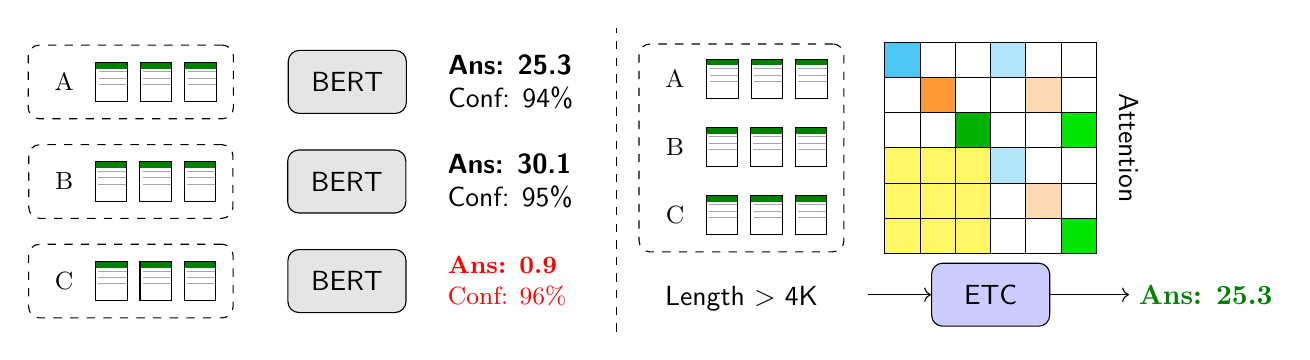
\begin{tikzpicture}[
  font=\sffamily,
  bert/.style={draw, rounded corners, fill=gray!20, minimum width=1.5cm, minimum height=0.8cm},
  dashedbox/.style={draw, dashed, rounded corners, inner sep=6pt},
  nobox/.style={draw=none, fill=none, inner sep=0pt},
  doc/.style={draw, fill=white, minimum width=0.4cm, minimum height=0.5cm, path picture={
    % green top bar
    \fill[green!50!black] (path picture bounding box.north west) rectangle ++(0.4cm,-0.08cm);
    % inner lines (simulating document text)
    \draw[gray!70, line width=0.2pt] ([xshift=1pt,yshift=-0.12cm]path picture bounding box.north west)
      -- ++(0.36cm,0);
    \draw[gray!70, line width=0.2pt] ([xshift=1pt,yshift=-0.2cm]path picture bounding box.north west)
      -- ++(0.36cm,0);
    \draw[gray!70, line width=0.2pt] ([xshift=1pt,yshift=-0.28cm]path picture bounding box.north west)
      -- ++(0.36cm,0);
  }},
  etc/.style={draw, rounded corners, fill=blue!20, minimum width=1.5cm, minimum height=0.8cm},
  label/.style={font=\small},
  confgood/.style={label, text=black},
  confbad/.style={label, text=red}
]

% A block
\node[label] (A) {A};
\node[doc, right=0.15cm of A] (Ad1) {};
\node[doc, right=0.15cm of Ad1] (Ad2) {};
\node[doc, right=0.15cm of Ad2] (Ad3) {};
\node [dashedbox, fit=(A)(Ad1)(Ad2)(Ad3)] (Abox) {};
\node[bert, right=0.9cm of Ad3] (BERTa) {BERT};
\node[align=left, right=0.4cm of BERTa] {
  \textbf{Ans: 25.3} \\ Conf: 94\%
};

% B block
\node[label, below=0.8cm of A] (B) {B};
\node[doc, right=0.15cm of B] (Bd1) {};
\node[doc, right=0.15cm of Bd1] (Bd2) {};
\node[doc, right=0.15cm of Bd2] (Bd3) {};
\node [dashedbox, fit=(B)(Bd1)(Bd2)(Bd3)] (Bbox) {};
\node[bert, right=0.9cm of Bd3] (BERTb) {BERT};
\node[align=left, right=0.4cm of BERTb] {
  \textbf{Ans: 30.1} \\ Conf: 95\%
};

% C block
\node[label, below=0.8cm of B] (C) {C};
\node[doc, right=0.15cm of C] (Cd1) {};
\node[doc, right=0.15cm of Cd1] (Cd2) {};
\node[doc, right=0.15cm of Cd2] (Cd3) {};
\node [dashedbox, fit=(C)(Cd1)(Cd2)(Cd3)] (Cbox) {};
\node[bert, right=0.9cm of Cd3] (BERTc) {BERT};
\node[align=left, confbad, right=0.4cm of BERTc] (ans3){
  \textbf{Ans: \textcolor{red}{0.9}} \\ Conf: 96\%
};

%global left box
\node [nobox, fit=(Abox)(ans3)] (globalbox) {};

% Vertical dashed separator
\draw[dashed] ([xshift=0.5cm, yshift=-0.2cm]globalbox.south east) -- ([xshift=0.5cm, yshift=0.2cm]globalbox.north east);

% Duplicate of documents
% AA block
\node[label, right=of globalbox.north east, anchor=north west, yshift=-6pt] (AA) {A};
\node[doc, right=0.15cm of AA] (AAd1) {};
\node[doc, right=0.15cm of AAd1] (AAd2) {};
\node[doc, right=0.15cm of AAd2] (AAd3) {};

% BB block
\node[label, below=0.4cm of AA] (BB) {B};
\node[doc, right=0.15cm of BB] (BBd1) {};
\node[doc, right=0.15cm of BBd1] (BBd2) {};
\node[doc, right=0.15cm of BBd2] (BBd3) {};

% CC block
\node[label, below=0.4cm of BB] (CC) {C};
\node[doc, right=0.15cm of CC] (CCd1) {};
\node[doc, right=0.15cm of CCd1] (CCd2) {};
\node[doc, right=0.15cm of CCd2] (CCd3) {};

\node[dashedbox, fit=(AA)(CCd3)] (globalbox2) {};
\node[below= 0.3cm of globalbox2] (Length) {Length $>$ 4K};
%
% Attention matrix
\node[nobox, right= 0.5cm of globalbox2] (att) {
\begin{adjustbox}{width=2.7cm, height=2.7cm, keepaspectratio}
  \begin{tabular}{|c|c|c|c|c|c|}
  \hline
  \cellcolor{cyan!70}&&&\cellcolor{cyan!30}&&\\
  \hline
  &\cellcolor{orange!80}&&&\cellcolor{orange!30}&\\
  \hline
  &&\cellcolor{green!70!black}&&&\cellcolor{green!90!black}\\
  \hline
  \cellcolor{yellow!60}&\cellcolor{yellow!60}&\cellcolor{yellow!60}&\cellcolor{cyan!30}&&\\
  \hline
  \cellcolor{yellow!60}&\cellcolor{yellow!60}&\cellcolor{yellow!60}&&\cellcolor{orange!30}&\\
  \hline
  \cellcolor{yellow!60}&\cellcolor{yellow!60}&\cellcolor{yellow!60}&&&\cellcolor{green!90!black}\\
  \hline
  \end{tabular}
  \end{adjustbox}
};
\node[rotate=-90, anchor=south] at ([xshift=0.15cm]att.east) {Attention};

% ETC box and output
\node[etc, below=0.1cm of att] (ETC) {ETC};
\node[font=\bfseries, text=green!50!black, right=1cm of ETC](Ans) {Ans: 25.3};
\draw[->] ([xshift = -0.8cm]ETC.west) -- (ETC.west);
\draw[->] (ETC.east) -- (Ans.west);

\end{tikzpicture}
\caption{\textbf{Left:} Single-block reader with input shorter than 512 tokens (baseline). \textbf{Right:} Cross-block reader with length over 4K tokens, and \=A denotes the global state assigned to local block A. The single-block reader is stuck at local optimum, while cross-block reader outputs global optimum.}
\end{figure}

\end{document}
